%
%===============>>  ГРУППА 11-2 МОДУЛЬ 6  <<=============
%
\setmodule{6}

%BEGIN_FOLD % ====>>_____ Занятие 1 _____<<====
\begin{class}[number=1]
	\begin{listofex}
		\item Площадь грани прямоугольного параллелепипеда равна \( 15 \). Ребро, перпендикулярное этой грани, равно \(3\). Найдите объем параллелепипеда.
		\item Три ребра прямоугольного параллелепипеда, выходящие из одной вершины, равны \(4, 6, 9\). Найдите ребро равновеликого ему куба.
		\item Два ребра прямоугольного параллелепипеда, выходящие из одной вершины, равны \(3\) и \(4\). Площадь поверхности этого параллелепипеда равна \(94\). Найдите третье ребро, выходящее из той же вершины.
		\item Прямоугольный параллелепипед описан около сферы радиуса \(1\). Найдите его площадь поверхности.
		\item Диагональ куба равна \( 2\sqrt{3} \). Найдите объем куба и площадь его поверхности.
		\item Объем первого куба в \( 8 \) раз больше объема второго куба. Во сколько раз площадь поверхности первого куба больше площади поверхности второго куба?
		\item Найдите площадь боковой поверхности правильной шестиугольной призмы, сторона основания которой равна \( 5 \), а высота  --- \( 10 \).
		\item Дан куб \( ABCDA_1B_1C_1D_1 \). Площадь четырехугольника \( ABC_1D_1 \) равна \( 4\sqrt{2} \). Найдите площадь поверхности куба.
		\item 
		\begin{minipage}[t]{\bodywidth}
			В правильной треугольной пирамиде \(SABC\) с вершиной \(S\) биссектрисы треугольника \(ABC\) пересекаются в точке \(O\). Площадь треугольника \(ABC\) равна \(2\); объем пирамиды равен \(6\). Найдите длину отрезка \(OS\).
		\end{minipage}
		\hspace{0.02\linewidth}
		\begin{minipage}[t]{\picwidth}
			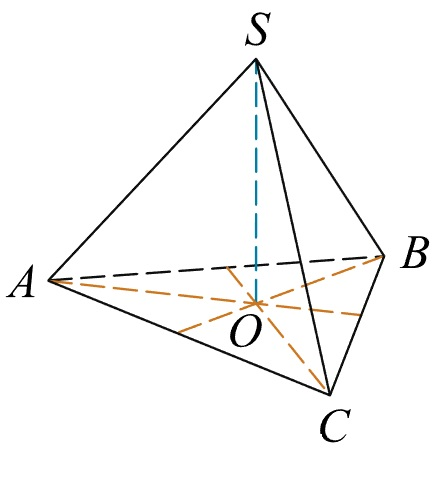
\includegraphics[align=t, width=\linewidth]{\picpath/G111M6L1-1}
		\end{minipage}
		\item В правильной четырехугольной пирамиде \(SABCD\) точка \(O\) --- центр основания, \(S\) --- вершина, \(SO=15, BD=16\). Найдите боковое ребро \(SA\).
		\item Объем параллелепипеда \(ABCDA_1B_1C_1D_1\) равен \(9\). Найдите объем треугольной пирамиды \(ABCA_1\).
		\item Во сколько раз увеличится объем правильного тетраэдра, если все его ребра увеличить в два раза?
		\item Первая цилиндрическая кружка вдвое выше второй, зато вторая в полтора раза шире. Найдите отношение объема второй кружки к объему первой. (Задание из пробника, вариант \( 1 \)).
		\item Сторона основания правильной шестиугольной пирамиды равна \( 3 \), боковое ребро равно \( 6 \).	Найдите объем пирамиды. (Задание из пробника, вариант \( 2 \)).
		\item Объём треугольной призмы, отсекаемой от куба плоскостью, проходящей через середины двух рёбер, выходящих из одной вершины, и параллельной третьему ребру, выходящему из	этой же вершины, равен \( 4 \). Найдите объём куба. (Задание из пробника, вариант \( 3 \)).
		\item Решите уравнения:
		\begin{tasks}(2)
			\task \( \sin x=\dfrac{1}{2} \)
			\task \( \cos x=-\dfrac{\sqrt{3}}{2} \)
			\task \( \sin x = -\dfrac{\sqrt{2}}{2} \)
			\task \( \tg x = \dfrac{-\sqrt{3}}{3} \)
			\task \( \ctg x = -1 \)
			\task \( \cos x = \dfrac{\sqrt{2}}{2} \)
		\end{tasks}
		\item Решить уравнения:
		\begin{tasks}(2)
			\task \( \cos\left( 2x+\dfrac{\pi}{4} \right)=\dfrac{\sqrt{2}}{2} \)
			\task \( \sin \left( 2x-\dfrac{3\pi}{2} \right) = -1 \)
			\task \( \cos \left( \dfrac{\pi}{4}-x \right)=\dfrac{\sqrt{3}}{2} \)
			\task \( \ctg\left( 2x-\dfrac{3\pi}{4} \right)=-1 \)
		\end{tasks}
	\end{listofex}
\end{class}
%END_FOLD

%BEGIN_FOLD % ====>>_____ Занятие 2 _____<<====
\begin{class}[number=2]
	\begin{listofex}
		\item Занятие 2
	\end{listofex}
\end{class}
%END_FOLD

%BEGIN_FOLD % ====>>_ Домашняя работа 1 _<<====
\begin{homework}[number=1]
	\begin{listofex}
		\item Решите уравнения:
		\begin{tasks}(2)
			\task \( \sin \left( x+\dfrac{\pi}{4} \right) = \dfrac{1}{2} \)
			\task \( \tg \left( 3x-\dfrac{12\pi}{7} \right) = -1 \)
			\task \( \cos \left( \dfrac{5\pi}{8}+x \right) = \dfrac{\sqrt{2}}{2} \)
		\end{tasks}
		\item Объем прямоугольного параллелепипеда равен \(24\). Одно из его ребер равно \(3\). Найдите площадь грани параллелепипеда, перпендикулярной этому ребру.
		\item 
		\begin{minipage}[t]{\bodywidth}
			В правильной треугольной пирамиде \(SABC\) точка \(M\) --- середина ребра \(AB\), \(S\) --- вершина. Известно, что \(BC = 3\), а площадь боковой поверхности пирамиды равна \(45\). Найдите длину отрезка \(SM\).
		\end{minipage}
		\hspace{0.02\linewidth}
		\begin{minipage}[t]{\picwidth}
			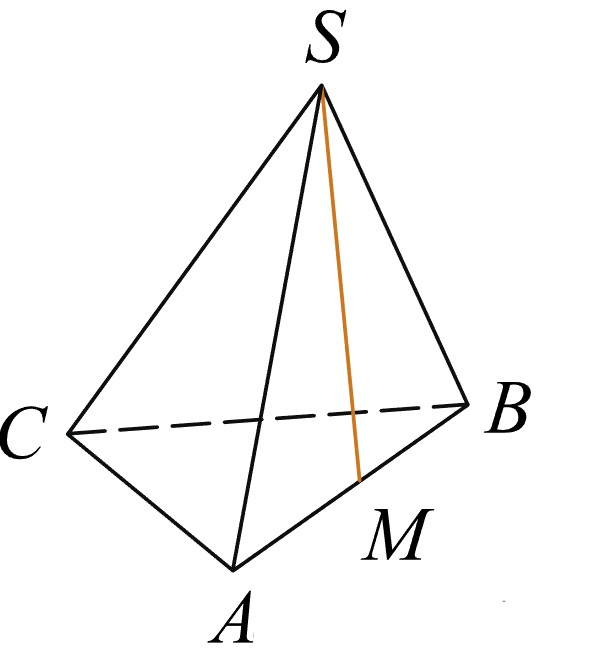
\includegraphics[align=t, width=\linewidth]{\picpath/G111M6L1-2}
		\end{minipage}
	\end{listofex}
\end{homework}
%END_FOLD

%BEGIN_FOLD % ====>>_____ Занятие 3 _____<<====
\begin{class}[number=3]
	\begin{listofex}
		\item Занятие 3 
	\end{listofex}
\end{class}
%END_FOLD

%BEGIN_FOLD % ====>>_____ Занятие 4 _____<<====
\begin{class}[number=4]
	\begin{listofex}
		\item Занятие 4
	\end{listofex}
\end{class}
%END_FOLD

%BEGIN_FOLD % ====>>_ Домашняя работа 2 _<<====
\begin{homework}[number=2]
	\begin{listofex}
		\item Домашняя работа 2
	\end{listofex}
\end{homework}
%END_FOLD

%BEGIN_FOLD % ====>>_____ Занятие 5 _____<<====
\begin{class}[number=5]
	\begin{listofex}
		\item Занятие 5
	\end{listofex}
\end{class}
%END_FOLD

%BEGIN_FOLD % ====>>_____ Занятие 6 _____<<====
\begin{class}[number=6]
	\begin{listofex}
		\item Занятие 6
	\end{listofex}
\end{class}
%END_FOLD

%BEGIN_FOLD % ====>>_ Домашняя работа 3 _<<====
\begin{homework}[number=3]
	\begin{listofex}
		\item Домашняя работа 3
	\end{listofex}
\end{homework}
%END_FOLD

%BEGIN_FOLD % ====>>_____ Занятие 7 _____<<====
\begin{class}[number=7]
	\title{Подготовка к проверочной}
	\begin{listofex}
		\item Занятие 7
	\end{listofex}
\end{class}
%END_FOLD

%BEGIN_FOLD % ====>>_ Проверочная работа _<<====
\begin{exam}
	\begin{listofex}
		\item Проверочная
	\end{listofex}
\end{exam}
%END_FOLD